\begin{minipage}{0.75\linewidth}
\begin{figure}[h]
    \centering
    \begin{adjustbox}{max width=1.0\linewidth, keepaspectratio}
        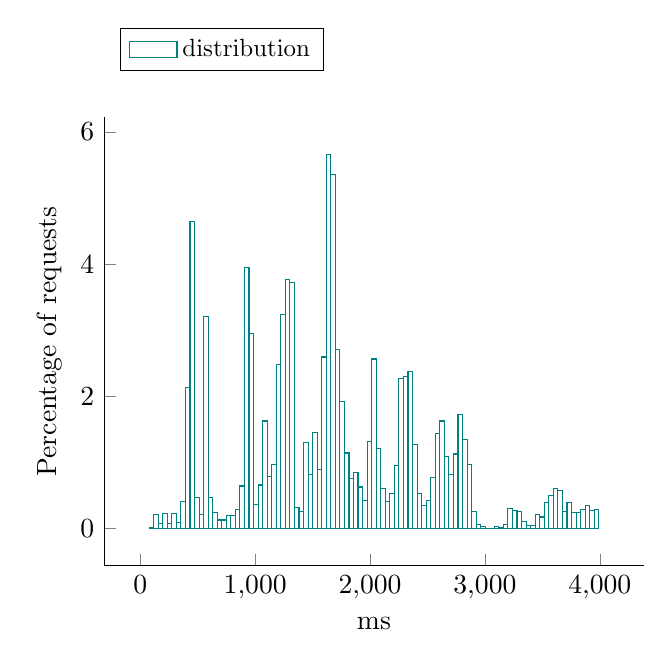
\begin{tikzpicture}
            \begin{axis}[ylabel = Percentage of requests, 
xlabel = ms, 
legend style = {nodes={scale=0.9, transform shape}, at={(0.03,1.2)}, anchor=north west, draw=black, fill=white, align=left, legend columns=3},
area style, mark size = 0pt,
 cycle list name = exotic,
  axis lines* = left]
		\addplot +[ybar interval] coordinates {
			 (76, 0.015625)
			 (115.55, 0.203125)
			 (155.1, 0.078125)
			 (194.65, 0.21875)
			 (234.2, 0.078125)
			 (273.75, 0.21875)
			 (313.3, 0.09375)
			 (352.85, 0.40625)
			 (392.4, 2.125)
			 (431.95, 4.64062)
			 (471.5, 0.46875)
			 (511.05, 0.203125)
			 (550.6, 3.20312)
			 (590.15, 0.46875)
			 (629.7, 0.234375)
			 (669.25, 0.125)
			 (708.8, 0.125)
			 (748.35, 0.1875)
			 (787.9, 0.1875)
			 (827.45, 0.28125)
			 (867, 0.640625)
			 (906.55, 3.95312)
			 (946.1, 2.95312)
			 (985.65, 0.359375)
			 (1025.2, 0.65625)
			 (1064.75, 1.625)
			 (1104.3, 0.78125)
			 (1143.85, 0.96875)
			 (1183.4, 2.48438)
			 (1222.95, 3.23437)
			 (1262.5, 3.76562)
			 (1302.05, 3.71875)
			 (1341.6, 0.3125)
			 (1381.15, 0.25)
			 (1420.7, 1.29688)
			 (1460.25, 0.8125)
			 (1499.8, 1.45312)
			 (1539.35, 0.890625)
			 (1578.9, 2.59375)
			 (1618.45, 5.65625)
			 (1658, 5.35938)
			 (1697.55, 2.70312)
			 (1737.1, 1.92188)
			 (1776.65, 1.14062)
			 (1816.2, 0.75)
			 (1855.75, 0.84375)
			 (1895.3, 0.625)
			 (1934.85, 0.421875)
			 (1974.4, 1.3125)
			 (2013.95, 2.5625)
			 (2053.5, 1.20312)
			 (2093.05, 0.609375)
			 (2132.6, 0.40625)
			 (2172.15, 0.53125)
			 (2211.7, 0.953125)
			 (2251.25, 2.26562)
			 (2290.8, 2.29688)
			 (2330.35, 2.375)
			 (2369.9, 1.26562)
			 (2409.45, 0.53125)
			 (2449, 0.34375)
			 (2488.55, 0.421875)
			 (2528.1, 0.765625)
			 (2567.65, 1.4375)
			 (2607.2, 1.625)
			 (2646.75, 1.09375)
			 (2686.3, 0.8125)
			 (2725.85, 1.125)
			 (2765.4, 1.71875)
			 (2804.95, 1.34375)
			 (2844.5, 0.96875)
			 (2884.05, 0.25)
			 (2923.6, 0.0625)
			 (2963.15, 0.03125)
			 (3002.7, 0)
			 (3042.25, 0)
			 (3081.8, 0.03125)
			 (3121.35, 0.015625)
			 (3160.9, 0.0625)
			 (3200.45, 0.296875)
			 (3240, 0.265625)
			 (3279.55, 0.25)
			 (3319.1, 0.109375)
			 (3358.65, 0.046875)
			 (3398.2, 0.046875)
			 (3437.75, 0.203125)
			 (3477.3, 0.171875)
			 (3516.85, 0.390625)
			 (3556.4, 0.5)
			 (3595.95, 0.609375)
			 (3635.5, 0.578125)
			 (3675.05, 0.25)
			 (3714.6, 0.390625)
			 (3754.15, 0.234375)
			 (3793.7, 0.234375)
			 (3833.25, 0.28125)
			 (3872.8, 0.34375)
			 (3912.35, 0.265625)
			 (3951.9, 0.28125)
			 (3991.45, 0.078125)
		};
\addlegendentry{distribution};
           \end{axis}
      \end{tikzpicture}
  \end{adjustbox}
  \caption{Response time distribution - req = ReadTimeline-0}
\end{figure}
\end{minipage}\hfill\begin{minipage}{0.18\linewidth}
\begin{table}[h]
\begin{tabular}{|cc|}
\hline
\textbf{} & \textbf{ms}\\ \hline
 \Xhline{0.005\arrayrulewidth}
min & 76\\
 \Xhline{0.005\arrayrulewidth}
max & 4031\\
 \Xhline{0.005\arrayrulewidth}
mean & 1702\\
 \Xhline{0.005\arrayrulewidth}
std & 825\\
\hline
\hline
 \Xhline{0.005\arrayrulewidth}
25th & 1168\\
 \Xhline{0.005\arrayrulewidth}
50th & 1645\\
 \Xhline{0.005\arrayrulewidth}
75th & 2282\\
 \Xhline{0.005\arrayrulewidth}
80th & 2364\\
 \Xhline{0.005\arrayrulewidth}
85th & 2607\\
 \Xhline{0.005\arrayrulewidth}
90th & 2771\\
 \Xhline{0.005\arrayrulewidth}
95th & 3326\\
 \Xhline{0.005\arrayrulewidth}
99th & 3870\\
\hline
\end{tabular}
\caption{Response time}
\end{table}
\end{minipage}\hfill